\infolevone{
\section{Superconducting Magnet Controls}
\label{sec:spectrometercontrols}
% Following text from Mike Fowler

The Hall C superconducting magnets, power supplies, and cryogenics are
controlled using two redundant pair Programmable Logic Controllers
(PLC). The PLC's are located on the second floor of the Counting
House. They are connected to the the magnets through hot swap analog
and digital IO modules. The IO modules for the High Momentum
Spectrometer (HMS) are also located on the second floor of the
Counting House while the IO modules for the Super High Momentum
Spectrometer (SHMS) are located in the electronics hut on the SHMS
structure in Hall C.

The operator interacts with the controls using the Human Machine
Interface (HMI) console located in the Hall C control room. The HMI
graphically displays the magnet status and allows the operator monitor
the magnet status, adjust the power supply, cryogenics, and remotely
rotate the spectrometers.  Example screens are shown in
Figs.~\ref{fig:magc_overview}, \ref{fig:magc_ESR_Data},
\ref{fig:magc_SHMS_Transfer_Line}, \ref{fig:magc_q1}
\ref{fig:magc_coilvoltages}, \ref{fig:magc_valves}, 
\ref{fig:magc_PowerSupply}, \ref{fig:magc_Nitrogen},
\ref{fig:magc_Helium}, 
\ref{fig:magc_q1forces} and \ref{fig:magc_Interlock},

Follow these instructions to operate the Hall C magnets.
\begin{itemize}
\item Type the command \mycomp{go\_cmagnets} from from one of the Hall
C counting house console computers.
\item Click on the ``Magnet Controls'' icon.
\item Click on the ``Status'' button to bring up an overview screen
for the magnets for both spectrometers.  The spectrometers may be set
``by momentum'' from this screen.
\item For individual magnet control, select the desired magnet and
click the ``PSU'' button.  Most power supply functions including setting
current, changing polarity, and resetting interlocks can be done from
these screens.
\item To remotely change spectrometer angles, click the ``Rotation'' button.
\end{itemize}
Other screens are availabe to show the status of cryogenics, and
forces and voltages within the magnets.  Control of cryogenic valves may
only be done under the direction of the engineer on call or other
member of the Hall C engineering group.



% Bunch of sample control screens from Mike Fowler  2/8/2016

\begin{figure}
\begin{center}
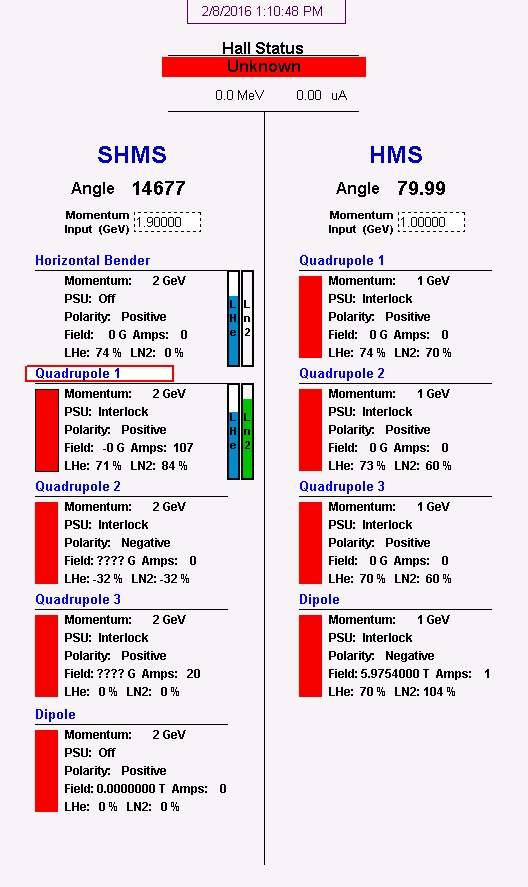
\includegraphics[width=0.7\textwidth]{new_overview}
\caption{\label{fig:magc_overview}Overview of HMS and SHMS magnet status}
\end{center}
\end{figure}

\begin{figure}
\begin{center}
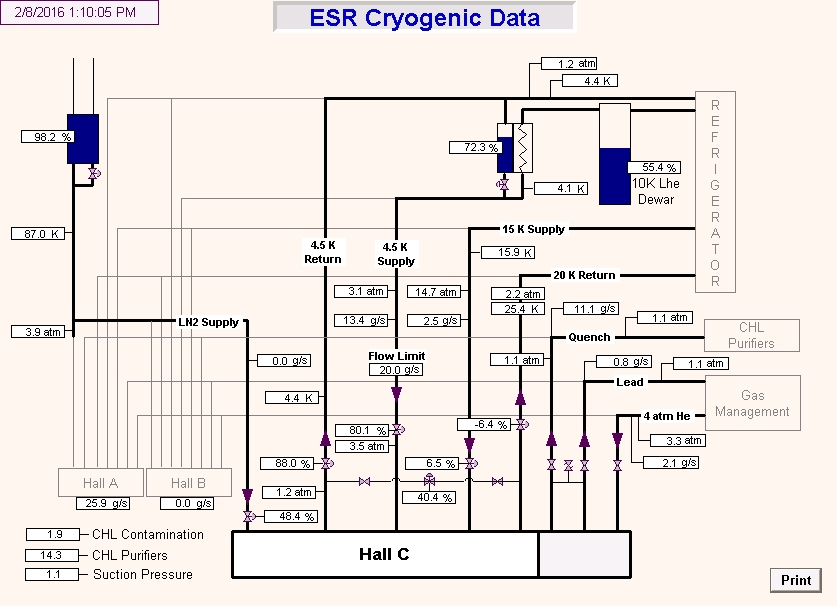
\includegraphics[width=0.9\textwidth]{new_ESR_Data}
\caption{\label{fig:magc_ESR_Data}Status of ESR Cryogenic System}
\end{center}
\end{figure}

\begin{figure}
\begin{center}
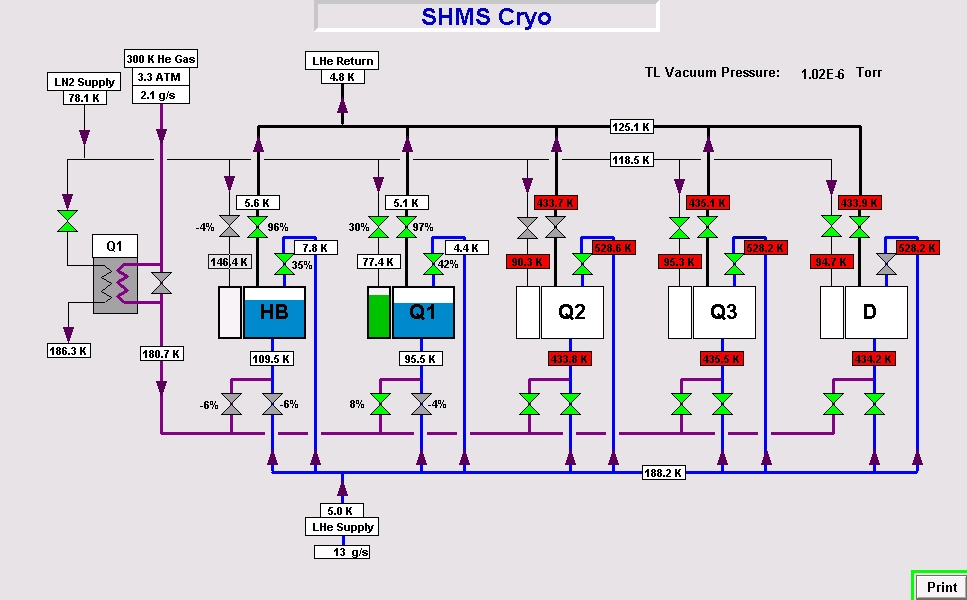
\includegraphics[width=0.9\textwidth]{new_SHMS_Transfer_Line}
\caption{\label{fig:magc_SHMS_Transfer_Line}SHMS Transfer Line}
\end{center}
\end{figure}

\begin{figure}
\begin{center}
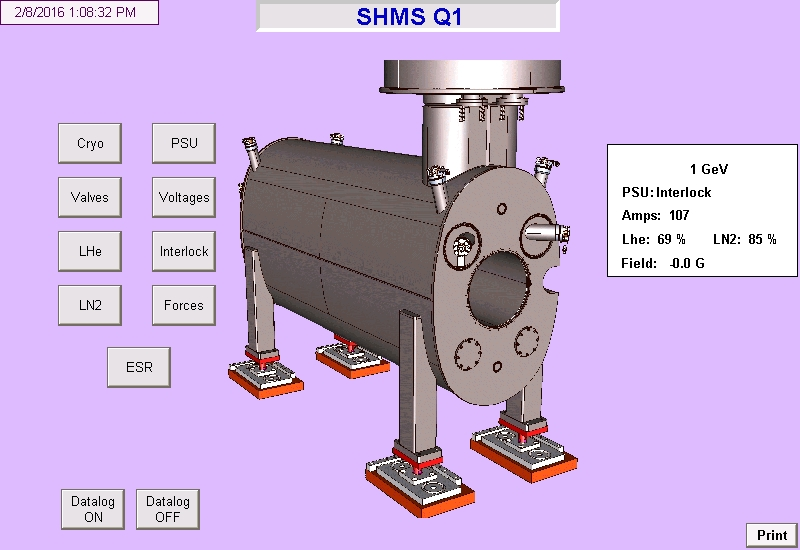
\includegraphics[width=0.9\textwidth]{new_Q1}
\caption{\label{fig:magc_q1}SHMS Q1 menu screen}
\end{center}
\end{figure}

\begin{figure}
\begin{center}
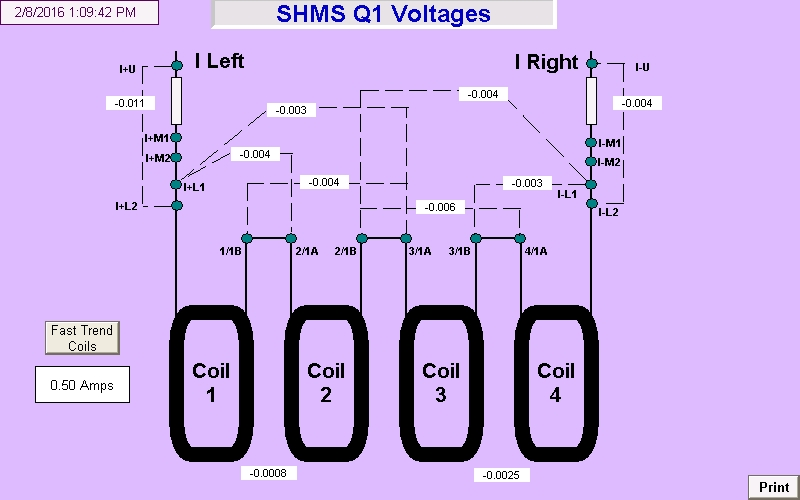
\includegraphics[width=0.9\textwidth]{new_CoilVoltages}
\caption{\label{fig:magc_coilvoltages}SHMS Q1 voltage taps.}
\end{center}
\end{figure}

\begin{figure}
\begin{center}
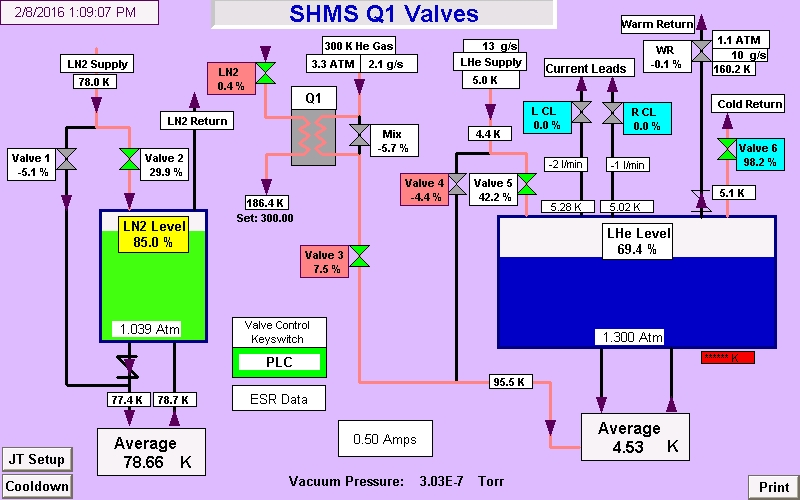
\includegraphics[width=0.9\textwidth]{new_Valves}
\caption{\label{fig:magc_valves}SHMS Q1 Valves}
\end{center}
\end{figure}

\begin{figure}
\begin{center}
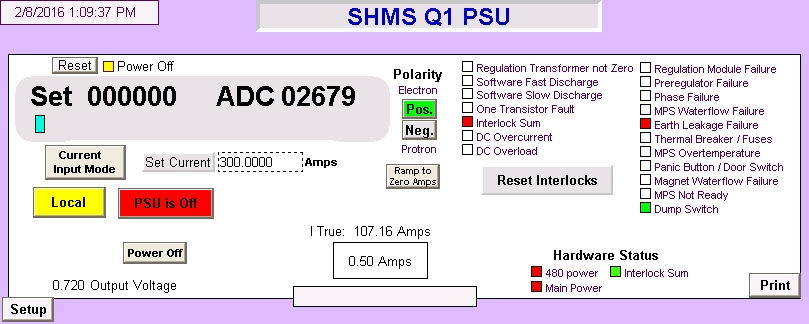
\includegraphics[width=0.9\textwidth]{new_PowerSupply}
\caption{\label{fig:magc_PowerSupply}}
\end{center}
\end{figure}

\begin{figure}
\begin{center}
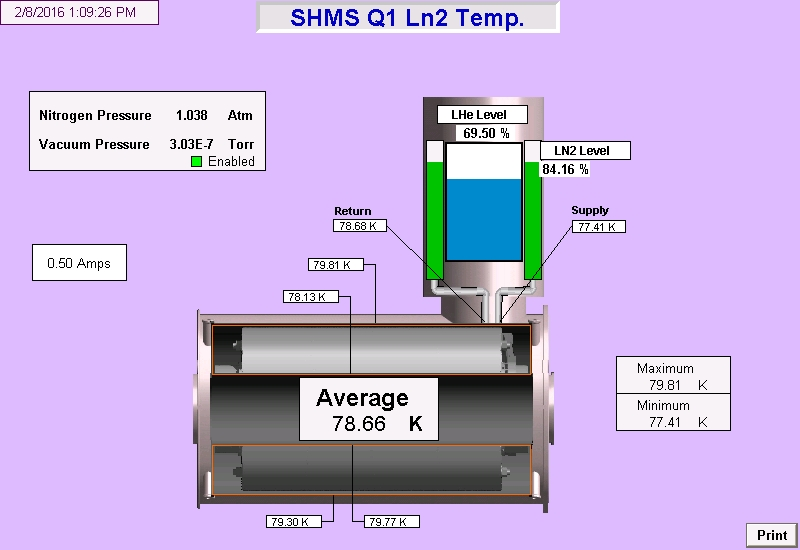
\includegraphics[width=0.9\textwidth]{new_Nitrogen}
\caption{\label{fig:magc_Nitrogen}SHMS Q1 nitrogen temperature and levels}
\end{center}
\end{figure}

\begin{figure}
\begin{center}
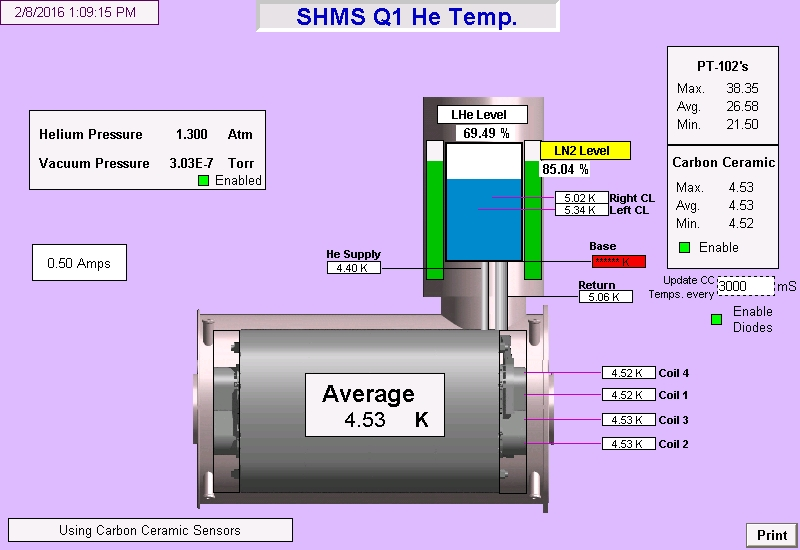
\includegraphics[width=0.9\textwidth]{new_Helium}
\caption{\label{fig:magc_Helium}SHMS Q1 helium temperatures and levels}
\end{center}
\end{figure}

\begin{figure}
\begin{center}
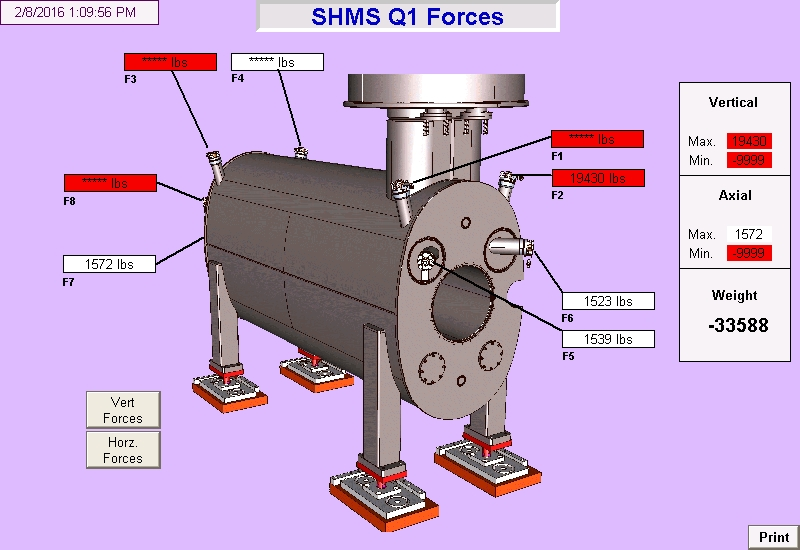
\includegraphics[width=0.9\textwidth]{new_Forces}
\caption{\label{fig:magc_q1forces}Forces on SHMS Q1 coil packs}
\end{center}
\end{figure}

\begin{figure}
\begin{center}
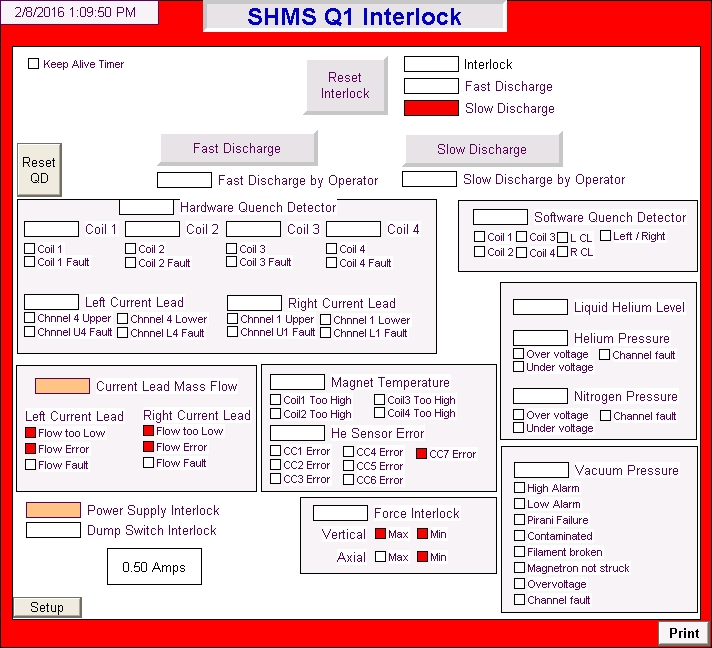
\includegraphics[width=0.9\textwidth]{new_Interlock}
\caption{\label{fig:magc_Interlock}SHMS Q1 power supply interlock status}
\end{center}
\end{figure}


\subsection{Responsible Personnel}
The PLCs are programed by and maintained by the Hall C engineering
staff.  In case of problems with spectrometer magnet and spectrometer
rotation controls, qualified personnel should be notified
(See Table~\ref{tab:spec:personnel_controls}).

\begin{namestab}{tab:spec:personnel_controls}{Spectrometers: authorized personnel}{%
      List of spectrometer responsible personnel where ``W.B.'' stands for the white board
      in the counting house.}
   \SteveLassiter{}
   \AmyComer{}
%   \EricSun{}
\end{namestab}

} %\infolevone
